\documentclass[border=5pt]{standalone}
\usepackage[T1]{fontenc}
\usepackage{lmodern,amsmath}
\usepackage[american]{circuitikz}
\usetikzlibrary{arrows.meta}
\begin{document}
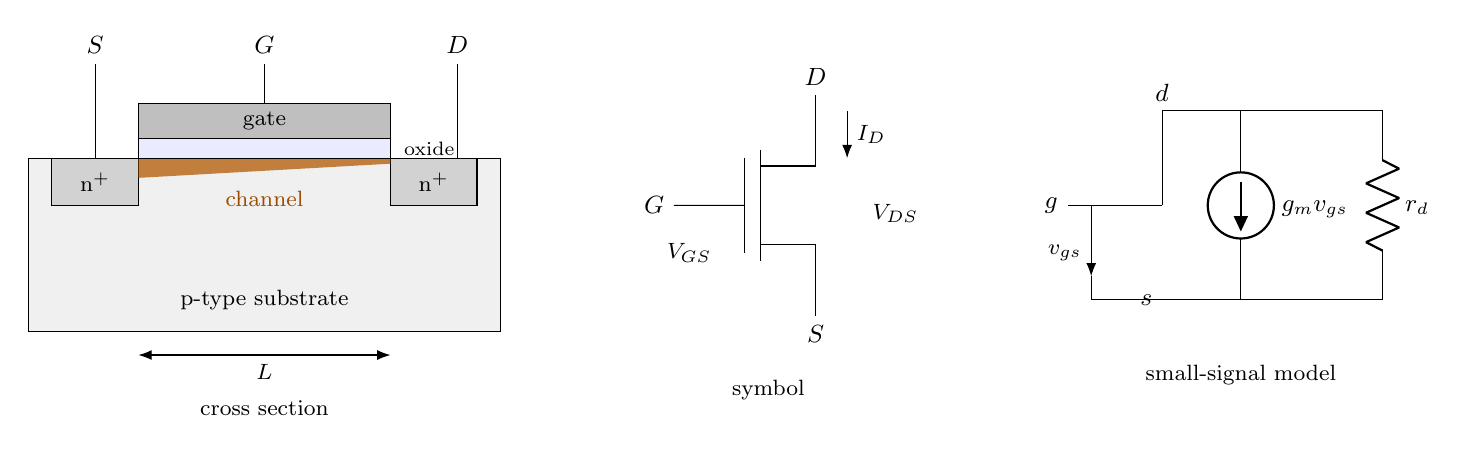
\begin{tikzpicture}[font=\small,>=Latex]
% left: cross section
\fill[gray!12] (0,0) rectangle (6,2.2);
\draw (0,0) rectangle (6,2.2);
\node[font=\footnotesize] at (3,0.4) {p-type substrate};
\fill[gray!35] (0.3,1.6) rectangle (1.4,2.2); \draw (0.3,1.6) rectangle (1.4,2.2);
\fill[gray!35] (4.6,1.6) rectangle (5.7,2.2); \draw (4.6,1.6) rectangle (5.7,2.2);
\node[font=\footnotesize] at (0.85,1.9) {n$^+$};
\node[font=\footnotesize] at (5.15,1.9) {n$^+$};
\fill[orange!70!black,opacity=.75] (1.4,2.2) -- (4.6,2.2) -- (4.6,2.13) -- (1.4,1.95) -- cycle;
\node[font=\footnotesize,orange!60!black,anchor=north] at (3,1.9) {channel};
\fill[blue!8] (1.4,2.2) rectangle (4.6,2.45); \draw (1.4,2.2) rectangle (4.6,2.45);
\node[font=\scriptsize,anchor=west] at (4.65,2.32) {oxide};
\fill[gray!50] (1.4,2.45) rectangle (4.6,2.9); \draw (1.4,2.45) rectangle (4.6,2.9);
\node[font=\footnotesize] at (3,2.67) {gate};
\draw (0.85,2.2) -- (0.85,3.4) node[above]{$S$};
\draw (3,2.9) -- (3,3.4) node[above]{$G$};
\draw (5.45,2.2) -- (5.45,3.4) node[above]{$D$};
\draw[<->] (1.4,-0.3) -- (4.6,-0.3) node[midway,below,font=\footnotesize]{$L$};
\node[font=\footnotesize,anchor=north] at (3,-0.75) {cross section};
% middle: symbol
\begin{scope}[xshift=8.2cm,yshift=0.6cm]
\draw (0,1) node[left]{$G$} to[short] (0.9,1);
\draw (0.9,0.4) -- (0.9,1.6);
\draw (1.1,0.3) -- (1.1,1.7);
\draw (1.1,1.5) -- (1.8,1.5) -- (1.8,2.4) node[above]{$D$};
\draw (1.1,0.5) -- (1.8,0.5) -- (1.8,-0.4) node[below]{$S$};
\draw[->] (2.2,2.2) -- (2.2,1.6) node[midway,right,font=\footnotesize]{$I_D$};
\node[font=\footnotesize,anchor=north] at (1.2,-1.1) {symbol};
\node[font=\footnotesize,anchor=west] at (2.4,0.9) {$V_{DS}$};
\node[font=\footnotesize,anchor=east] at (0.6,0.4) {$V_{GS}$};
\end{scope}
% right: small-signal model
\begin{scope}[xshift=13.2cm,yshift=0.2cm]
\draw (0,1.4) node[left]{$g$} -- (1.2,1.4);
\draw (1.2,2.6) node[above]{$d$} -- (1.2,1.4);
\draw (1.2,2.6) -- (2.2,2.6) to[isource, l=$g_m v_{gs}$] (2.2,0.2) -- (1.2,0.2);
\draw (2.2,2.6) -- (4.0,2.6) to[R, l=$r_d$] (4.0,0.2) -- (2.2,0.2);
\draw (1.2,0.2) node[left]{$s$} -- (1.2,0.2);
\draw[->] (0.3,1.1) -- (0.3,0.5) node[midway,left,font=\footnotesize]{$v_{gs}$};
\draw (0.3,1.4) -- (0.3,1.1); \draw (0.3,0.5) -- (0.3,0.2) -- (1.2,0.2);
\node[font=\footnotesize,anchor=north] at (2.2,-0.5) {small-signal model};
\end{scope}
\end{tikzpicture}
\end{document}
